\documentclass{article}
\usepackage{tikz}
\usetikzlibrary{positioning}
\usetikzlibrary{calc}
\usetikzlibrary{arrows,shapes,backgrounds}
\begin{document}


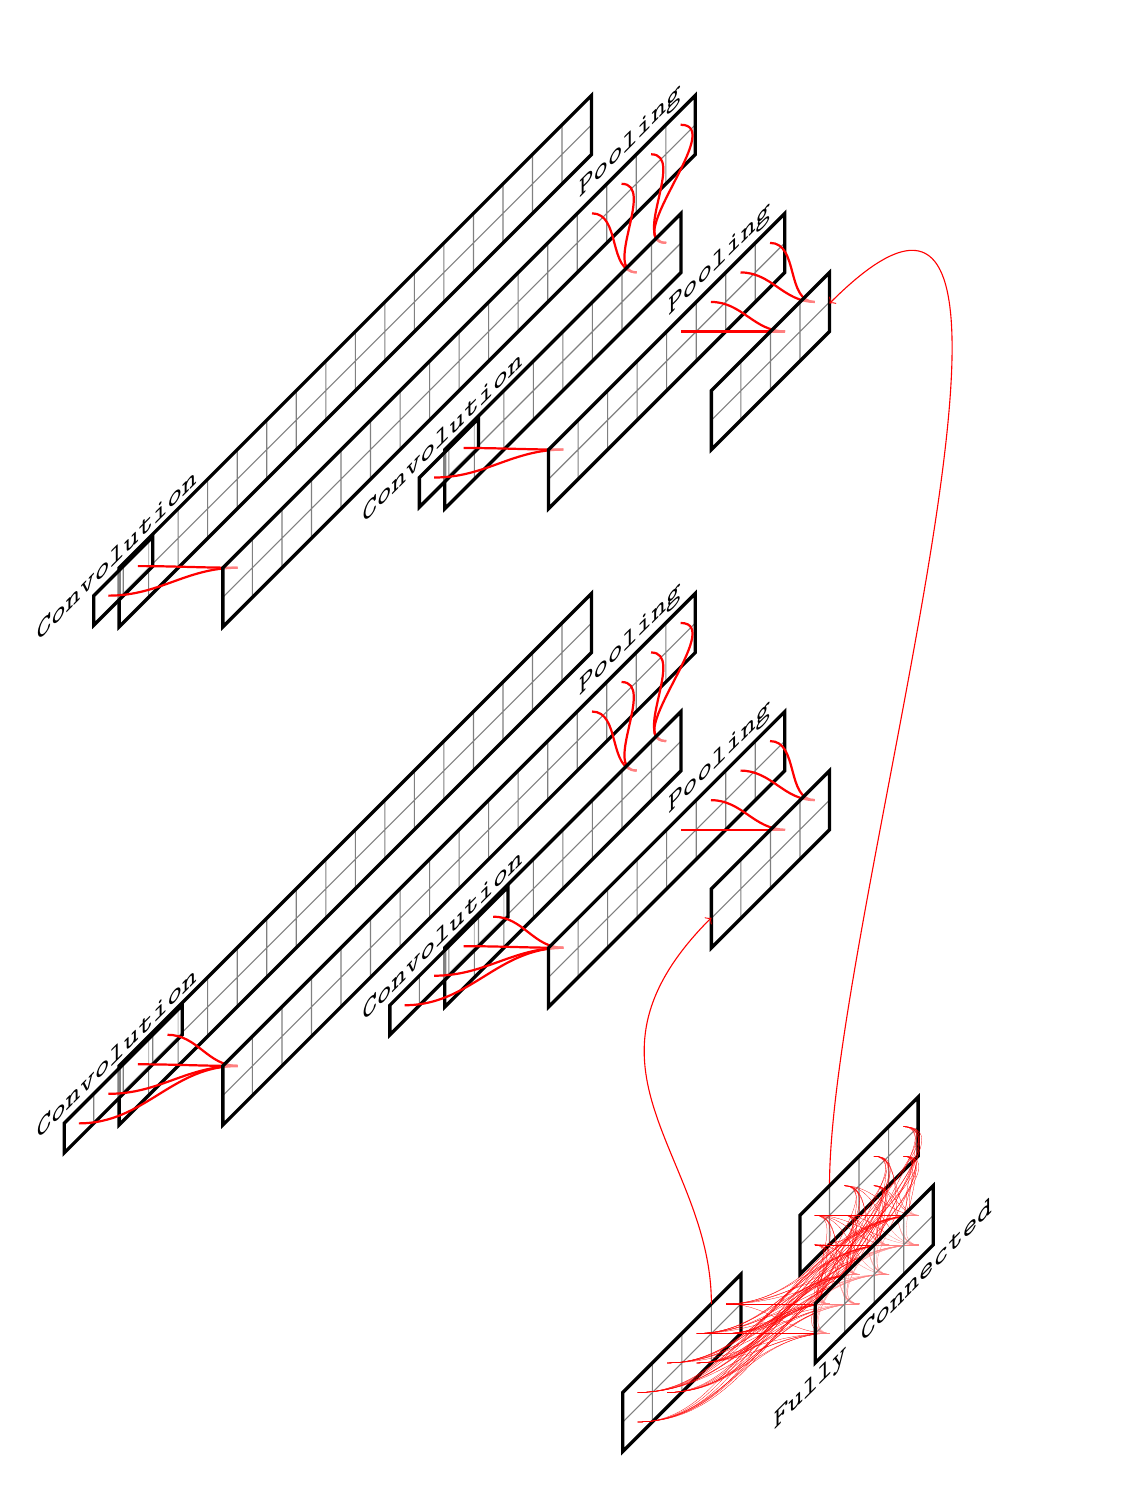
\begin{tikzpicture}[scale=1.5,every node/.style={minimum size=1cm},on grid]
\foreach \yshift in {120, 0}{
    \begin{scope}[
            yshift=\yshift, xshift=-100, every node/.append style={
            yslant=1,xslant=0},yslant=1,xslant=0]
        \fill[white,fill opacity=0.9] (0,0) rectangle (4,0.5);
        \draw[step=2.5mm, thin, gray] (0,0) grid (4,0.5); %defining grids
        \draw[black,very thick] (0,0) rectangle (4,0.5);%marking borders      
		\pgfkeys{/pgf/number format/.cd, fixed, zerofill, precision =1} 
    \end{scope}
    
    \begin{scope}[
            yshift=\yshift+7.5, xshift=-99, every node/.append style={
            yslant=1,xslant=0},yslant=1,xslant=0]
            
        \ifnum 0=\yshift {
        \fill[white,fill opacity=0.5] (-0.5,0) rectangle (0.5,0.25);
        \draw[step=2.5mm, thin, gray] (-0.5,0) grid (0.5,0.25); %defining grids
        \draw[black,very thick] (-0.5,0) rectangle (0.5,0.25);%marking borders     
		}\fi
		
        \ifnum 120=\yshift {
        \fill[white,fill opacity=0.5] (-0.25,0) rectangle (0.25,0.25);
        \draw[step=2.5mm, thin, gray] (-0.25,0) grid (0.25,0.25); %defining grids
        \draw[black,very thick] (-0.25,0) rectangle (0.25,0.25);%marking borders     
		}\fi
        
        \coordinate (sphi1) at (-3*0.25/2,0.25/2);
        \coordinate (sphi2) at (-1*0.25/2,0.25/2);
        \coordinate (sphi3) at (1*0.25/2,0.25/2);
        \coordinate (sphi4) at (3*0.25/2,0.25/2);
        \fill[black]
		node at ([yshift=8, xshift=2]sphi2) {\texttt{Convolution}};
    \end{scope}

    \begin{scope}[
            yshift=\yshift, xshift=-75, every node/.append style={
            yslant=1,xslant=0},yslant=1,xslant=0]
		\coordinate (spho1) at (1*0.25/2,3*0.25/2);
		\coordinate (sphob1) at (25*0.25/2,3*0.25/2);
		\coordinate (spho2) at (27*0.25/2,3*0.25/2);
		\coordinate (spho3) at (29*0.25/2,3*0.25/2);
		\coordinate (spho4) at (31*0.25/2,3*0.25/2);
        \fill[black]
		node at ([yshift=8, xshift=2]spho2) {\texttt{Pooling}};
	\end{scope}

\draw[thick,red](sphi2)
        to[out=0,in=180] (spho1);
\draw[thick,red](sphi3)
        to[out=0,in=180] (spho1);

        
\ifnum 0=\yshift {
\draw[thick,red](sphi1)
        to[out=0,in=180] (spho1);
\draw[thick,red](sphi4)
        to[out=0,in=180] (spho1);
}\fi

    \begin{scope}[
            yshift=\yshift, xshift=-75, every node/.append style={
            yslant=1,xslant=0},yslant=1,xslant=0]
        \fill[white,fill opacity=0.5] (0,0) rectangle (4,0.5);
        \draw[step=2.5mm, thin, gray] (0,0) grid (4,0.5); %defining grids
        \draw[black,very thick] (0,0) rectangle (4,0.5);%marking borders      
		%\node at (spho1) [fill=black,circle,scale=0.2] {$s$};
		\pgfkeys{/pgf/number format/.cd, fixed, zerofill, precision =1} 
    \end{scope}

    \begin{scope}[
            yshift=\yshift, xshift=-50, every node/.append style={
            yslant=1,xslant=0},yslant=1,xslant=0]
        \coordinate (sphh1) at (21*0.25/2,3*0.25/2);  
        \coordinate (sphh2) at (23*0.25/2,3*0.25/2);  
    \end{scope}
    
\draw[thick,red](sphob1)
        to[out=0,in=180] (sphh1);
\draw[thick,red](spho2)
        to[out=0,in=180] (sphh1);
\draw[thick,red](spho3)
        to[out=0,in=180] (sphh2);
\draw[thick,red](spho4)
        to[out=0,in=180] (sphh2);

    \begin{scope}[
            yshift=\yshift, xshift=-50, every node/.append style={
            yslant=1,xslant=0},yslant=1,xslant=0]
        \fill[white,fill opacity=0.5] (1,0) rectangle (3,0.5);
        \draw[step=2.5mm, thin, gray] (1,0) grid (3,0.5); %defining grids
        \draw[black,very thick] (1,0) rectangle (3,0.5);%marking borders    
		%\node at (sphi) [fill=black,circle,scale=0.2] {$s$};
		\pgfkeys{/pgf/number format/.cd, fixed, zerofill, precision =1} 
    \end{scope}
    
    \begin{scope}[
            yshift=\yshift+7.5, xshift=-49, every node/.append style={
            yslant=1,xslant=0},yslant=1,xslant=0]
            
 		
        \ifnum 0=\yshift {
        \fill[white,fill opacity=0.5] (1.5,0) rectangle (0.5,0.25);
        \draw[step=2.5mm, thin, gray] (1.5,0) grid (0.5,0.25); %defining grids
        \draw[black,very thick] (1.5,0) rectangle (0.5,0.25);%marking borders     
		}\fi
 
        \ifnum 120=\yshift {
        \fill[white,fill opacity=0.5] (1.25,0) rectangle (0.75,0.25);
        \draw[step=2.5mm, thin, gray] (1.25,0) grid (0.75,0.25); %defining grids
        \draw[black,very thick] (1.25,0) rectangle (0.75,0.25);%marking borders     
		}\fi
        
        \coordinate (sphi1) at (5*0.25/2,0.25/2);
        \coordinate (sphi2) at (7*0.25/2,0.25/2);
        \coordinate (sphi3) at (9*0.25/2,0.25/2);
        \coordinate (sphi4) at (11*0.25/2,0.25/2);
        
        \fill[black]
		node at ([yshift=8, xshift=2]sphi2) {\texttt{Convolution}};
    \end{scope}
    
    \begin{scope}[
            yshift=\yshift, xshift=-25, every node/.append style={
            yslant=1,xslant=0},yslant=1,xslant=0]
		\coordinate (spho1) at (9*0.25/2,3*0.25/2);
		\coordinate (sphob1) at (17*0.25/2,3*0.25/2);
		\coordinate (spho2) at (19*0.25/2,3*0.25/2);
		\coordinate (spho3) at (21*0.25/2,3*0.25/2);
		\coordinate (spho4) at (23*0.25/2,3*0.25/2);
        \fill[black]
		node at ([yshift=8, xshift=2]spho2) {\texttt{Pooling}};
	\end{scope}
	

\draw[thick,red](sphi2)
        to[out=0,in=180] (spho1);
\draw[thick,red](sphi3)
        to[out=0,in=180] (spho1);

\ifnum 0=\yshift {
\draw[thick,red](sphi1)
        to[out=0,in=180] (spho1);
\draw[thick,red](sphi4)
        to[out=0,in=180] (spho1);
}\fi

    \begin{scope}[
            yshift=\yshift, xshift=-25, every node/.append style={
            yslant=1,xslant=0},yslant=1,xslant=0]
        \fill[white,fill opacity=0.5] (1,0) rectangle (3,0.5);
        \draw[step=2.5mm, thin, gray] (1,0) grid (3,0.5); %defining grids
        \draw[black,very thick] (1,0) rectangle (3,0.5);%marking borders    
		%\node at (sphi) [fill=black,circle,scale=0.2] {$s$};
		\pgfkeys{/pgf/number format/.cd, fixed, zerofill, precision =1} 
    \end{scope}
    
    \begin{scope}[
            yshift=\yshift, xshift=0, every node/.append style={
            yslant=1,xslant=0},yslant=1,xslant=0]
        \coordinate (sphh1) at (17*0.25/2,3*0.25/2);  
        \coordinate (sphh2) at (19*0.25/2,3*0.25/2);  
    \end{scope}
    
\draw[thick,red](sphob1)
        to[out=0,in=180] (sphh1);
\draw[thick,red](spho2)
        to[out=0,in=180] (sphh1);
\draw[thick,red](spho3)
        to[out=0,in=180] (sphh2);
\draw[thick,red](spho4)
        to[out=0,in=180] (sphh2);
    
    \begin{scope}[
            yshift=\yshift, xshift=0, every node/.append style={
            yslant=1,xslant=0},yslant=1,xslant=0]
        \fill[white,fill opacity=0.5] (1.5,0) rectangle (2.5,0.5);
        \draw[step=2.5mm, thin, gray] (1.5,0) grid (2.5,0.5); %defining grids
        \draw[black,very thick] (1.5,0) rectangle (2.5,0.5);%marking borders    
		%\node at (sphi) [fill=black,circle,scale=0.2] {$s$};
		\pgfkeys{/pgf/number format/.cd, fixed, zerofill, precision =1} 
    \end{scope}
    
}

    \begin{scope}[
            yshift=-100, xshift=0, every node/.append style={
            yslant=1,xslant=0},yslant=1,xslant=0]
        \fill[white,fill opacity=0.5] (0.75,0) rectangle (1.75,0.5);
        \draw[step=2.5mm, thin, gray] (0.75,0) grid (1.75,0.5); %defining grids
        \draw[black,very thick] (0.75,0) rectangle (1.75,0.5);%marking borders    
		%\node at (sphi) [fill=black,circle,scale=0.2] {$s$};
		\pgfkeys{/pgf/number format/.cd, fixed, zerofill, precision =1} 
		\draw[->,red,looseness=0.8](2.5, 0.5) to [out=90,in=0] (2.5,7.97);
    \end{scope}
    
    \begin{scope}[
            yshift=-100, xshift=0, every node/.append style={
            yslant=1,xslant=0},yslant=1,xslant=0]
        \fill[white,fill opacity=0.5] (2.25,0) rectangle (3.25,0.5);
        \draw[step=2.5mm, thin, gray] (2.25,0) grid (3.25,0.5); %defining grids
        \draw[black,very thick] (2.25,0) rectangle (3.25,0.5);%marking borders    
		%\node at (sphi) [fill=black,circle,scale=0.2] {$s$};
		\pgfkeys{/pgf/number format/.cd, fixed, zerofill, precision =1} 
		\draw[->,red,looseness=1](1.5, 0.5) to [out=90,in=180] (1.5,3.77);
    \end{scope}

	\begin{scope}[yshift=-100]
        \foreach \xa in {3.5, 4.5, 5.5, 6.5, 9.5, 10.5, 11.5, 12.5}{
        	\foreach \ya in {0.5, 1.5}{
        		\foreach \xb in {6.5, 7.5, 8.5, 9.5}{
        			\foreach \yb in {0.5,1.5}{
                 		\draw[ultra thin,red,looseness=1]([yslant=1]\xa*0.25, \ya*0.25) to[out=0,in=180] ([yslant=1, xshift=25, yshift=-25]\xb*0.25,\yb*0.25);
                 	}
                }
            }
		}
	\end{scope}
	
    \begin{scope}[
            yshift=-100, xshift=25, every node/.append style={
            yslant=1,xslant=0},yslant=1,xslant=0]
        \fill[white,fill opacity=0.5] (1.5,0) rectangle (2.5,0.5);
        \draw[step=2.5mm, thin, gray] (1.5,0) grid (2.5,0.5); %defining grids
        \draw[black,very thick] (1.5,0) rectangle (2.5,0.5);%marking borders    
		%\node at (sphi) [fill=black,circle,scale=0.2] {$s$};
		\pgfkeys{/pgf/number format/.cd, fixed, zerofill, precision =1} 
		\fill[black]
		node at ([yshift=-5, xshift=59]0, 0) {\texttt{Fully Connected}};
    \end{scope}



\end{tikzpicture}
\end{document}
